\section{Usage}

\subsection{Browser requirements}

The application has been designed for use with Firefox.  For the best user experience a modern version of Firefox should be used.

The application has also been tested with Google Chrome.  When using Chrome all the functionality is available however the application runs considerably slower than Firefox.  If speed becomes an issue please consider using Firefox.

The application has not been tested with other browsers such as Edge, Internet Explorer or Safari.  While the application may function on these no guarantees are made.

\subsection{CSV}

The main application page can be found at the '/upload' endpoint.  This will be 'commute.napier.ac.uk/upload' if using the Napier University server or at '127.0.0.1/upload' if you are hosting the application locally.

On loading the application you will be presented by the view below (Figure \ref{img:csv-upload-page-layout}).

\begin{figure}[h]
	
\includegraphics[width=\linewidth]{images/csv-upload-page-layout.png}
	\caption{The first view presented by the application}
	\label{img:csv-upload-page-layout}
\end{figure}

This box may be clicked, or a CSV file dragged onto it, to initialise the application.  If the CSV file is incorrectly formatted the page may not present an error but may not function correctly.  Displaying or error messages will hopefully be added in a future update.

The application may appear to stall at this point.  It may stall for up to 1 minute depending on the size of the CSV file and the software and hardware used to access the site.

Once the CSV file is loaded you will be presented with a page similar to the following image (Figure \ref{img:csv-uploaded-page-layout}).  This page has been divided into four sub-section which are detailed below.

\begin{figure}[h]
	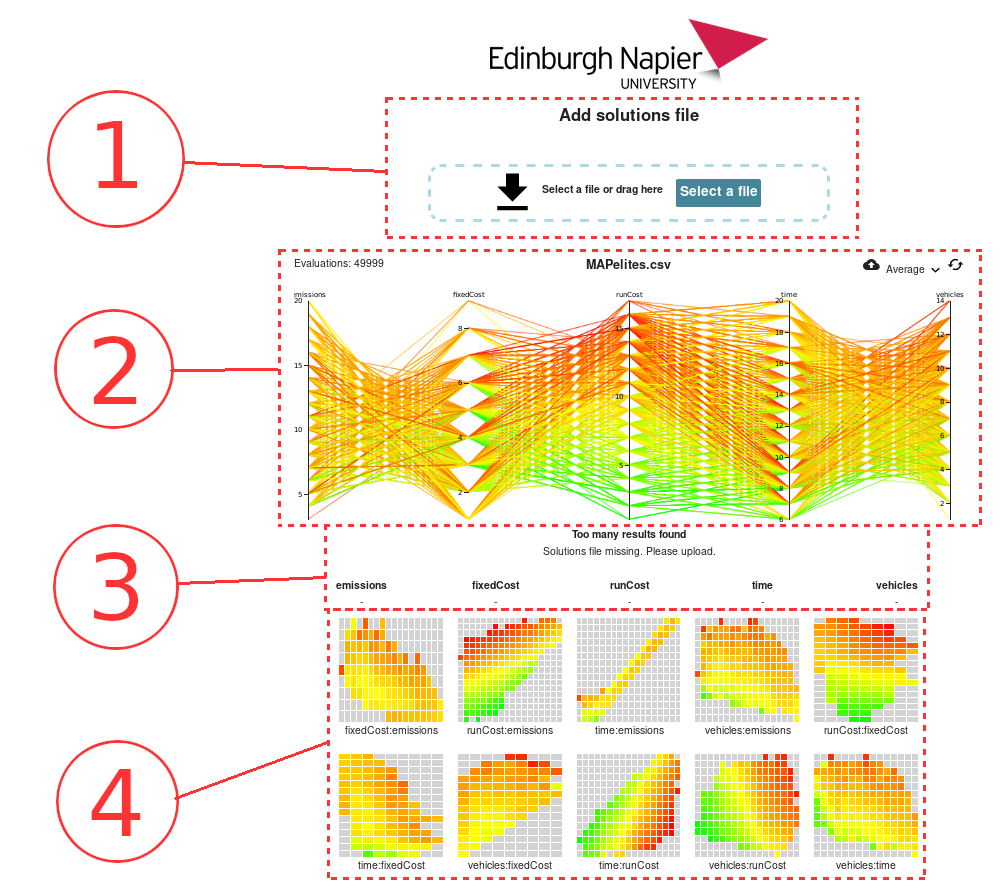
\includegraphics[width=\linewidth]{images/csv-uploaded-page-layout.png}
	\caption{The page layout when a valid CSV file has been uploaded}
	\label{img:csv-uploaded-page-layout}
\end{figure}

\subsubsection{Section 1 - Solution upload} \label{section:solutions-upload}

The first section allows the user to upload the zipped solutions folder mentioned in \ref{section:file-format-solutions-zip}.  This does not display when a solutions file has already been uploaded to the server.  In this event the section can be shown by clicking the cloud icon at the top right of section 2.  If a second file is uploaded this will overwrite the first file.

\paragraph{File locks}  Only one user may upload a solutions file for a specific CSV file at one time.  If another user attempts to upload a a file an error message will be displayed.  If an upload fails or is cancelled there is a chance this message will be displayed incorrectly.  This issues will automatically fix itself after 15 minutes.

Details of how to manually clear the locks can be found in the installation and maintenance documentation.

\subsubsection{Section 2 - Parallel coordinates}

The second section contains a parallel coordinates graph.

This graph is interactive and can be filtered by clicking or dragging on each of the columns.  Right clicking on a filtered column will reset it.  Clicking the refresh button in the top right will reset all the columns.

The graph is colour where red lines have a high distance and green lines have a low distance.

\subsubsection{Section 3 - Results}

The third section contains details about any selected results.  This section only displays information when a single solution is selected through the filtering in the parallel coordinates.  If this section contains the text 'Too many results found' then more than one result is available through the parallel coordinates filtering.

When a single result is found, the details of that result are displayed in this section.  If a solutions file has been uploaded the 'View details' link can be clicked to view further details loaded from the solutions zip file.  If this link leads to a 'Not found' page then the solutions file and the CSV file do not match and correct or updated solutions file should be uploaded as mentioned in \ref{section:solutions-upload}.

\subsubsection{Section 4 - Heatmaps}

Section 4 contains heatmaps to display the data.  These are filtered to display the same data at the parallel coordinates graph is section 2.

By default these heatmaps are coloured based on the average distance of all the elements on a tile.  This can be changed to use the best distance of the elements on a tile using the drop-down in the top right of section 2.
